\appendix
\chapter{Individual Constructions}

We diagram lethal set constructions for single grids. The initial infection $A$ is colored red, and all other cells are labeled with the time $t$ that they are first infected. 

\section{Perfect constructions}

% (5, 2, 2)
\begin{con}
\label{con:5x2x2}
The grid $(5,2,2)$ is perfect.
\end{con}

\begin{proof}
See figure \ref{fig:2x5x2_numbered_heatmap}.
\end{proof}

\begin{figure}[]
\centering
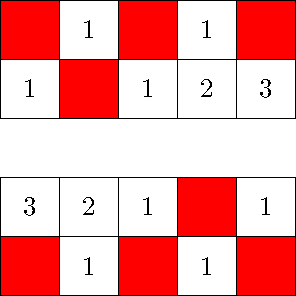
\includegraphics[width=0.2\textwidth]{figures/7/2x5x2_numbered_heatmap.pdf}
\caption{}
\label{fig:2x5x2_numbered_heatmap}
\end{figure} 

% (5, 5, 5)
\begin{con}
\label{con:5x5x5}
The grid $(5,5,5)$ is perfect.
\end{con}

\begin{proof}
See figure \ref{fig:5x5x5_numbered_heatmap}.
\end{proof}

\begin{figure}[]
\centering
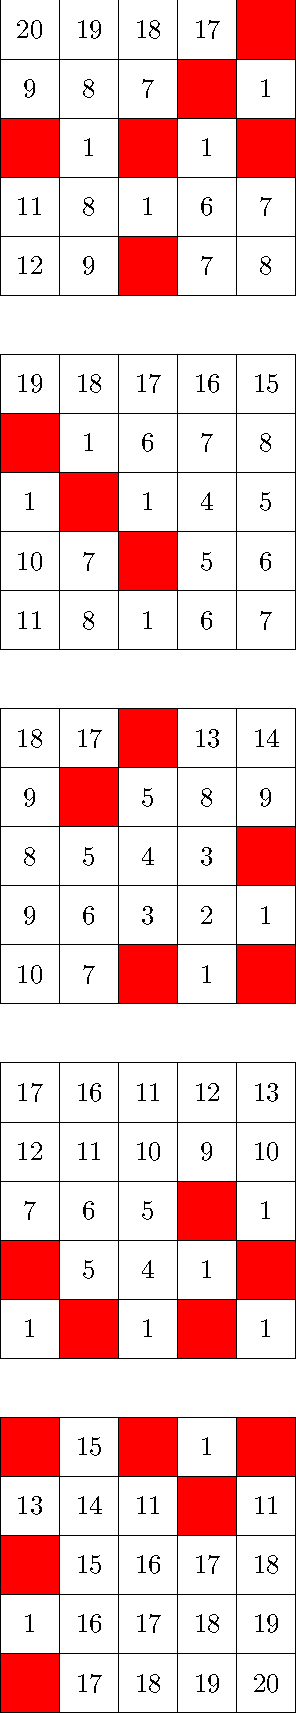
\includegraphics[width=0.2\textwidth]{figures/7/5x5x5_numbered_heatmap.pdf}
\caption{}
\label{fig:5x5x5_numbered_heatmap}
\end{figure}

% (8, 5, 5)
\begin{con}
\label{con:8x5x5}
The grid $(8,5,5)$ is perfect.
\end{con}

\begin{proof}
See figure \ref{fig:5x8x5_numbered_heatmap}.
\end{proof}

\begin{figure}[]
\centering
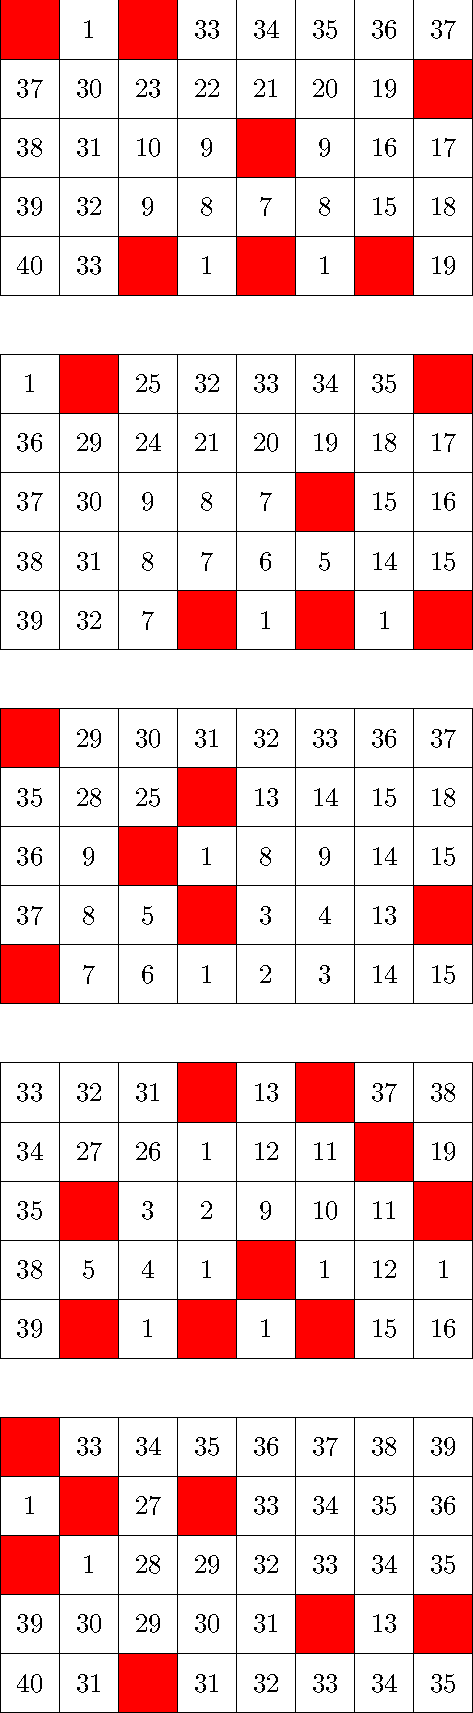
\includegraphics[width=0.2\textwidth]{figures/7/5x8x5_numbered_heatmap.pdf}
\caption{}
\label{fig:5x8x5_numbered_heatmap}
\end{figure}

% (9, 6, 5)
\begin{con}
\label{con:9x6x5}
The grid $(9,6,5)$ is perfect.
\end{con}

\begin{proof}
See figure \ref{fig:6x9x5_numbered_heatmap}.
\end{proof}

\begin{figure}[]
\centering
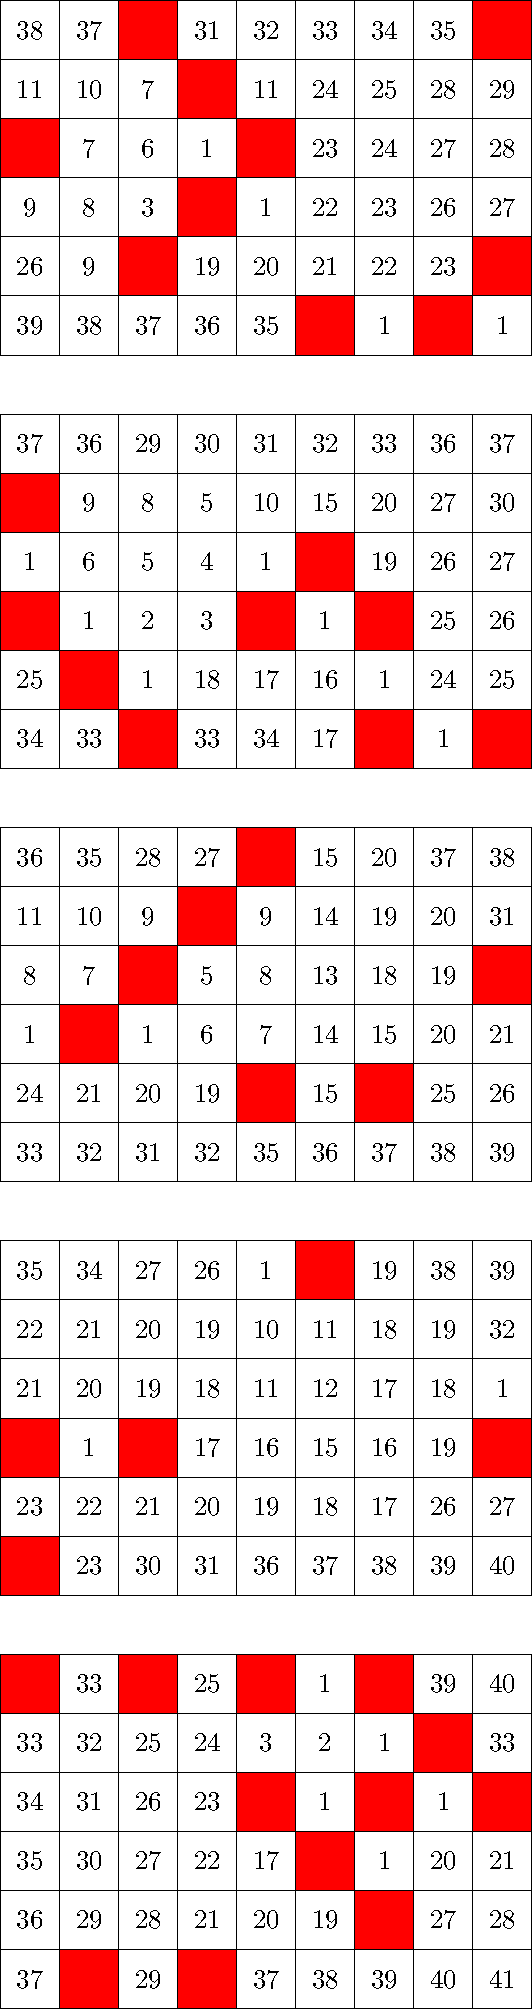
\includegraphics[width=0.2\textwidth]{figures/A/6x9x5_numbered_heatmap.pdf}
\caption{}
\label{fig:6x9x5_numbered_heatmap}
\end{figure}

% (5,5,2)
\begin{con}
\label{con:5x5x2}
The grid $(5,5,2)$ is perfect.
\end{con}

\begin{proof}
See figure \ref{fig:5x5x2_numbered_heatmap}.
\end{proof}

\begin{figure}[]
\centering
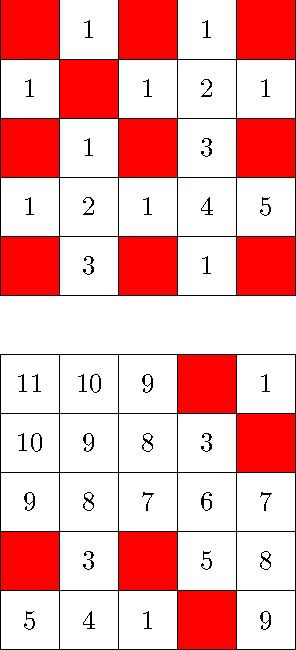
\includegraphics[width=0.2\textwidth]{figures/A/5x5x2_numbered_heatmap.pdf}
\caption{}
\label{fig:5x5x2_numbered_heatmap}
\end{figure}

% (2,2,2)
\begin{con}
\label{con:2x2x2}
The grid $(2,2,2)$ is perfect.
\end{con}

\begin{proof}
See figure \ref{fig:2x2x2_numbered_heatmap}.
\end{proof}

\begin{figure}[]
\centering
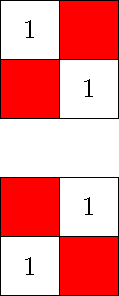
\includegraphics[width=0.2\textwidth]{figures/A/2x2x2_numbered_heatmap.pdf}
\caption{}
\label{fig:2x2x2_numbered_heatmap}
\end{figure}

% (6,4,3)
\begin{con}
\label{con:6x4x3}
The grid $(6,4,3)$ is perfect.
\end{con}

\begin{proof}
See figure \ref{fig:4x6x3_numbered_heatmap}.
\end{proof}

\begin{figure}[]
\centering
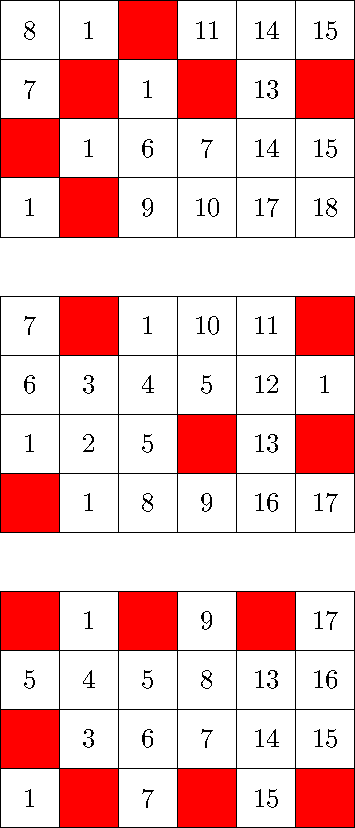
\includegraphics[width=0.2\textwidth]{figures/A/4x6x3_numbered_heatmap.pdf}
\caption{}
\label{fig:4x6x3_numbered_heatmap}
\end{figure}

% (3,3,1)
\begin{con}
\label{con:3x3x1}
The grid $(3,3,1)$ is perfect.
\end{con}

\begin{proof}
See figure \ref{fig:3x3x1_numbered_heatmap}.
\end{proof}

\begin{figure}[]
\centering
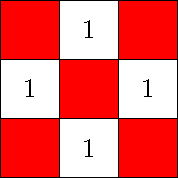
\includegraphics[width=0.2\textwidth]{figures/A/3x3x1_numbered_heatmap.pdf}
\caption{}
\label{fig:3x3x1_numbered_heatmap}
\end{figure}

% (3,3,3)
\begin{con}
\label{con:3x3x3}
The grid $(3,3,3)$ is perfect.
\end{con}

\begin{proof}
See figure \ref{fig:3x3x3_numbered_heatmap}.
\end{proof}

\begin{figure}[]
\centering
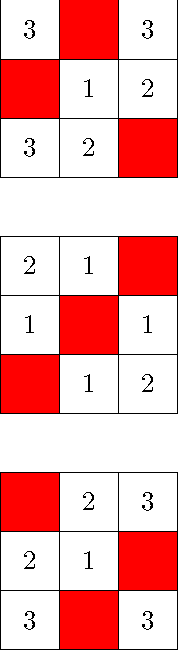
\includegraphics[width=0.2\textwidth]{figures/A/3x3x3_numbered_heatmap.pdf}
\caption{}
\label{fig:3x3x3_numbered_heatmap}
\end{figure}

\section{Optimal constructions}




